\documentclass[aspectratio=169]{beamer}
\usetheme{boxes}
\usepackage{essay-def}
\usepackage{bm}
\usepackage{amsfonts}
\usepackage{amssymb}
\usepackage{amsmath}
\usepackage{amsthm}
\usepackage{comment}
\usepackage{enumitem}
\usepackage{geometry}
\usepackage{subcaption}
\geometry{left=1cm,right=1cm}
    \title[Distribution Mismatch]{Combatting distribution shift in scientific machine learning}
\author[J. Zhao]{Jiaxi Zhao \\ \small joint with Q. Li \& S. Arisaka @ NUS, N. Thuerey @ TUM}
\date[\today]{9th NUS graduate symposium in mathematics \\ \today}
\begin{document}
\par \setlength{\parindent}{2em}

\begin{frame}
\titlepage
% TODO:for my thesis defense or presentation, may be it would be 
% good to discuss with qianxiao to check if my background slide is not too much

\end{frame}

\begin{frame}{Motivation:}
	Large-scale scientific simulations are unaffordable, e.g. 50M grids, 10s $\Longrightarrow$ 2 days.
	\begin{figure}[ht]
		\centering
		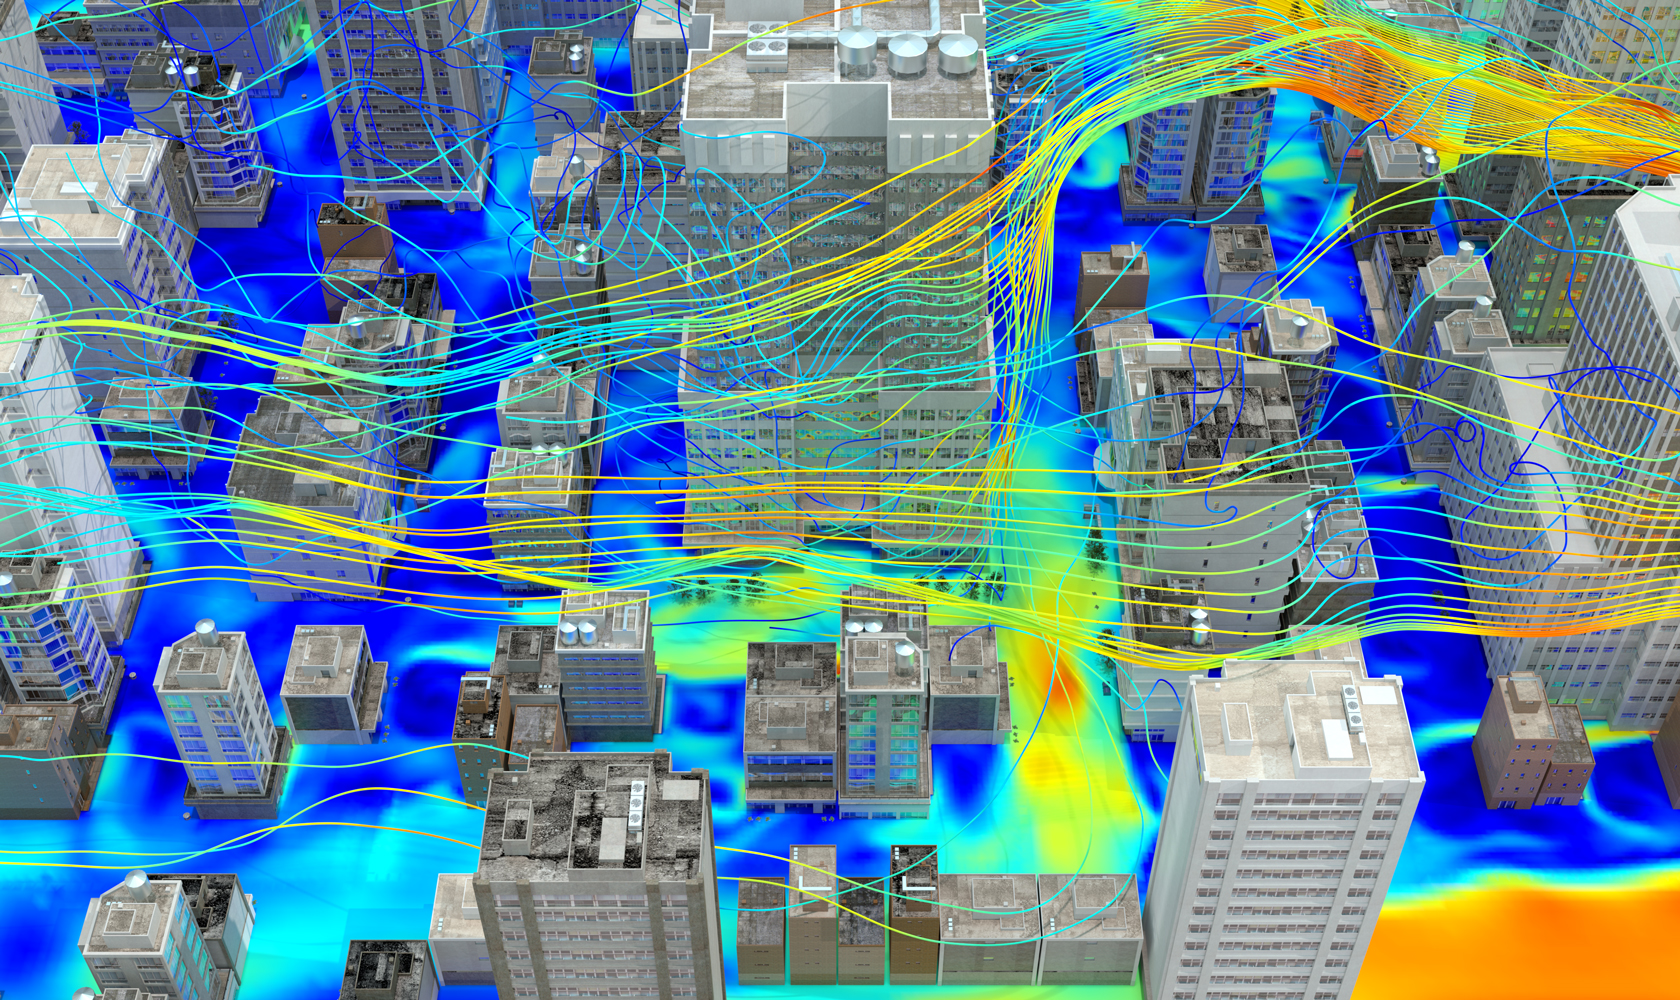
\includegraphics[width=.5\linewidth]{fig/urban_environment.jpeg}
	\end{figure}

	Data-driven modeling \textbf{\color{red} may} improve the simulations:
	\begin{itemize}
		\item 1. Reduced-order model.
		\item 2. Surrogate model.
	\end{itemize}
\end{frame}

\begin{frame}{An abstraction of SciML workflow}
	Simulating the dynamics:
	\bequn
		\begin{aligned}
			\mcL(\mfu, \p_t \mfu, \mfy, t) & = \mathbf{0}, \quad \mfu \in \mcU, \mfy \in \mcY, \mcL: \mcU \times T\mcU \times \mcY \times \mbR_+ \rightarrow \mbR^{n},			\\
			\mfy & = \phi(\mfu, t), \quad \phi: \mcU \times \mbR_+ \rightarrow \mfy.
		\end{aligned}
	\eequn
	\begin{itemize}
		\item 1. $\mcL$ is known, possibly non-linear, {\color{red}while $\phi$ is un-known.}
		\item 2. Datasets: $\lbb (\mfu_1, \mfy_1, t_1), (\mfu_2, \mfy_2, t_2), \cdots, (\mfu_N, \mfy_N, t_N )\rbb. $
		\item 3. {\color{red} Benchmark algorithm solves the ordinary least square:
		\bequn
			\arg\min_{\theta} \mbE \norml \mfy - \phi_{\theta}(\mfu, t) \normr^2.
		\eequn}
	\end{itemize}
	
	Typical examples: subgrid-scale modeling, reynolds stress modeling, exchange-correlation functional.

\end{frame}

% 1 hour talk
% \begin{frame}{Iterative scheme is ubiquitous}
% 	There are different levels of iterative methods in scientific application:
% 	\begin{itemize}
% 		\item 1. High level: iterative method for forward and inverse problem
% 			\begin{itemize}
% 				\item * Steady simulation: RANS.
% 				\item * Unsteady simulation: LES, Molecular dynamics.
% 				\item * Optimization for inverse problem: inverse scattering.
% 			\end{itemize}
% 		\item 2. Low level: iterative method to solve the linear system:
% 			\begin{itemize}
% 				\item * Jacobi, Gauss-Seidel, SOR etc.
% 				\item * Connjugate gradient, GMRES, BiCGSTAB etc.
% 				\item * Preconditioning, e.g. ILU, AMG etc.
% 			\end{itemize}
% 	\end{itemize}
% \end{frame}

\begin{frame}{Dilemma of data-driven scientific computing}
	In the data-driven scientific computing, \textcolor{red}{\textbf{dynamics structure}}
	can cause \textcolor{red}{\textbf{distribution mismatch}} between the training and testing data.
	\textcolor{red}{\textbf{The stability of the iterative scheme}} is different from classical numerical analysis, e.g.
	Lax equivalence theorem.
	\begin{figure}[H]
          \centering
          \centerline{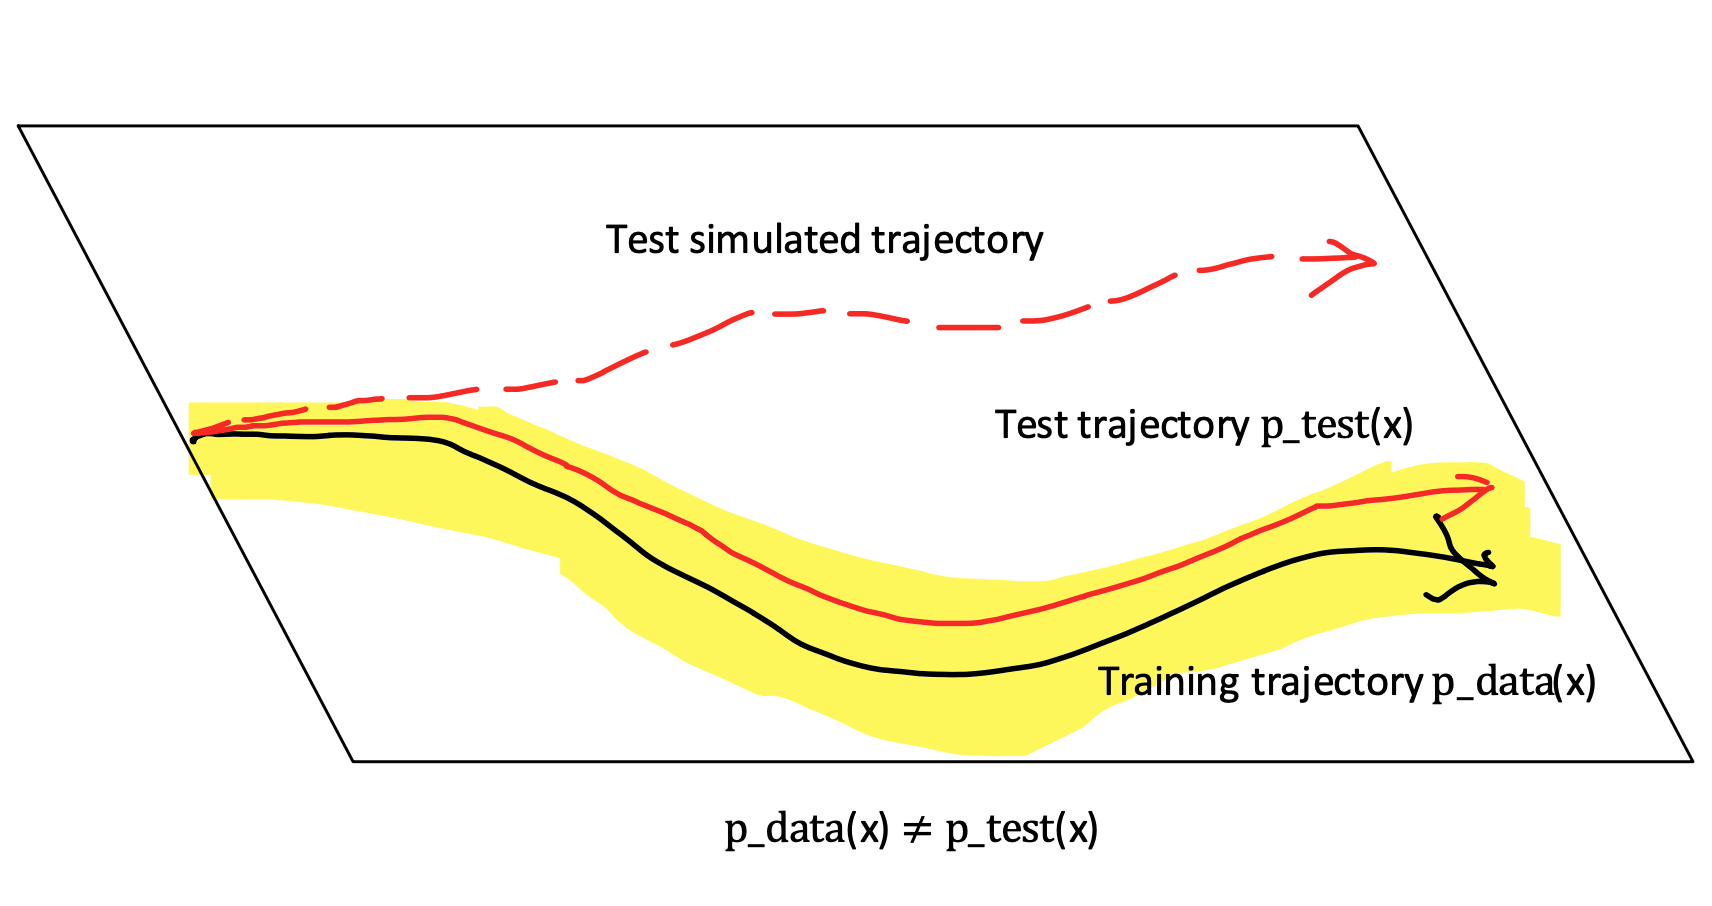
\includegraphics[width=.8\linewidth]{fig/dilemma.jpg}}
        \end{figure}
\end{frame}


% 1 hour talk
% \begin{frame}
% 	\begin{itemize}
% 		\item \textbf{Data generation:}
% 		\begin{itemize}
% 			\item Preprocessing, e.g. filterd DNS data compared with LES data
% 			\item Adaptive sampling \& Active learning
% 			\item Importance reweighting
% 		\end{itemize}
% 		\item \textbf{Learning algorithm:}
% 		\begin{itemize}
% 			\item Manifold-regularized learning
% 			\item Unrolled dynamics and reinforcement learning
% 		\end{itemize}
% 		\item \textbf{Simulated algorithm:}
% 		\begin{itemize}
% 			\item Subspace-aware algorithm
% 			\item Random subspace method
% 		\end{itemize}
% 	\end{itemize}
% \end{frame}

\begin{frame}{Manifold regularization}
	Regularization encodes the information of the data manifold.
	\begin{figure}[H]
		\centering
		\centerline{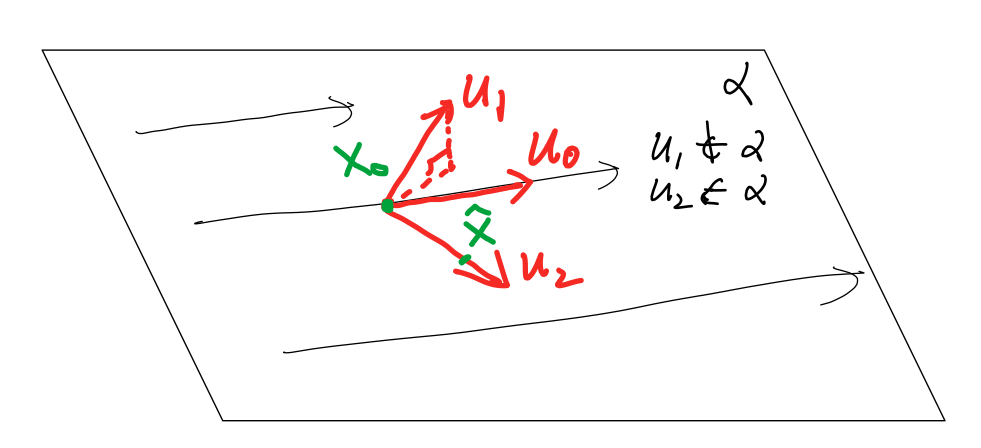
\includegraphics[width=0.9\linewidth]{fig/mfd.png}}
	\end{figure}
	\footnotetext[1]{Zhao, Jiaxi, and Qianxiao Li. "Mitigating Distribution Shift
	in Machine Learning–Augmented Hybrid Simulation." SIAM Journal on
	Scientific Computing 47.2 (2025): C475-C500.}
\end{frame}

% for optimization problem such as RANS
% \begin{frame}{The freedom of choosing simulated dynamics}
% 	For unsteady simulation problem, we can change the numerical scheme for simulation, i.e.
% 	spatial and temporal discretization. While for steady state simulation and inverse problem, we can 
% 	choose or design the numerical scheme:
% 	\begin{equation}
% 		\begin{aligned}
% 			\mathbf{0} & \ = \mcL_{\theta}(\mfu),	\\
% 		  \p_t \mfu & \ = \mcL_{\theta}(\mfu), \quad \text{(RANS simulation)}   \\
% 		  \p_t \mfu & \ = - \lp \nabla_u\mcL_{\theta}(\mfu) \rp^{-1} \mcL_{\theta}(\mfu) \quad \text{(Gauss Newton)}.
% 		\end{aligned}
% 	\end{equation}  
% 	The question is: \textit{How to go beyond linear?}
% \end{frame}

\begin{frame}{Linear dynamics}
	We consider the following the \text{\color{red}linear} hybrid simulation problem
	\bequn
		\begin{aligned}
			\frac{d\mfu}{dt} & = A\mfu + B\mfy,  \quad \mfu\in\mbR^m, \mfy \in \mbR^n, A\in \mbR^{m \times m}, B\in \mbR^{m \times n}   \\
			\mfy & = C^* \mfu,  \quad C^* \in \mbR^{n\times m}.
		\end{aligned}
	\eequn

	Assume the dynamics lie in a low-dimensional subspace $V$:
	\begin{equation*}
		l_{\text{TR}}(\wht C) := \mbE_{(\mfu, \mfy)} \lp \norml \wht C \mfu - \mfy \normr_2^2
		 + \lambda \norml P_{V^{\perp}}(A + B\wht C)\mfu \normr_2^2 \rp,
	\end{equation*}

	For nonlinear case, learn a function $F(\mfu)$ which has data manifold as a level set:
	\begin{equation*}
	l_{\text{TR}}(\theta) := \mbE_{(\mfu, \mfy)}\lb \norml \mfy_k - \phi_{\theta}(\mfu) \normr_2^2
	+ \lambda \lp\lp  \nabla F(\mfu) \rp^T L(\mfu, \phi_{\theta}(\mfu), t)\rp^2 \rb.
	\end{equation*}
\end{frame}

\begin{frame}{Design of regularization}
	The tangent-space regularized estimator has {\color{red}slower error scaling for large $\lambda$}:
	%#TODO: still need to think about how to present this part
	\begin{Thm}
		With $Q_m(r, T)$ defined by $m^2\int_0^T (2 + t^{m-1})e^{r t}dt$ and
		\begin{equation*}
			\begin{aligned}
				e_1 = \text{eig}_{\max}(A+B\wht C), \quad e_2 = \text{eig}_{\max}((A+B\wht C)P_V), \\
				\text{eig}_{\max}(A) = \max\{\Re(s): \exists v \neq \mathbf{0}, Av = sv\},
			\end{aligned}
		\end{equation*}
		the errors of OLS and our algorithm are bounded respectively by
		\begin{equation*}\label{equ:a-posterior-error}
			\begin{aligned}
				& \ \mbE\norml \wht\mfu_{\text{OLS}}(T) - \mfu(T) \normr \leq c_1\sqrt{\delta}\norml B \normr_2Q_m(e_1, T),      \\
				& \ \mbE\norml \wht\mfu_{\text{TR}}(T) - \mfu(T) \normr \leq c_2\sqrt{\delta}\Big(\norml B \normr_2 Q_m(e_2, T) \\
			& + \frac{9m^4c_3}{\sqrt{\lambda}}\lp 1 + 3m^2c_1\sqrt{\delta}\norml B \normr_2\rp\norml A+B\wht C \normr_2 (1\vee T^{3m})(1\vee e^{e_1T}) \Big).
			\end{aligned}
		\end{equation*}
	\end{Thm}
\end{frame}

\begin{frame}{Performance}
	\begin{figure}[ht]
		\centering
		\centerline{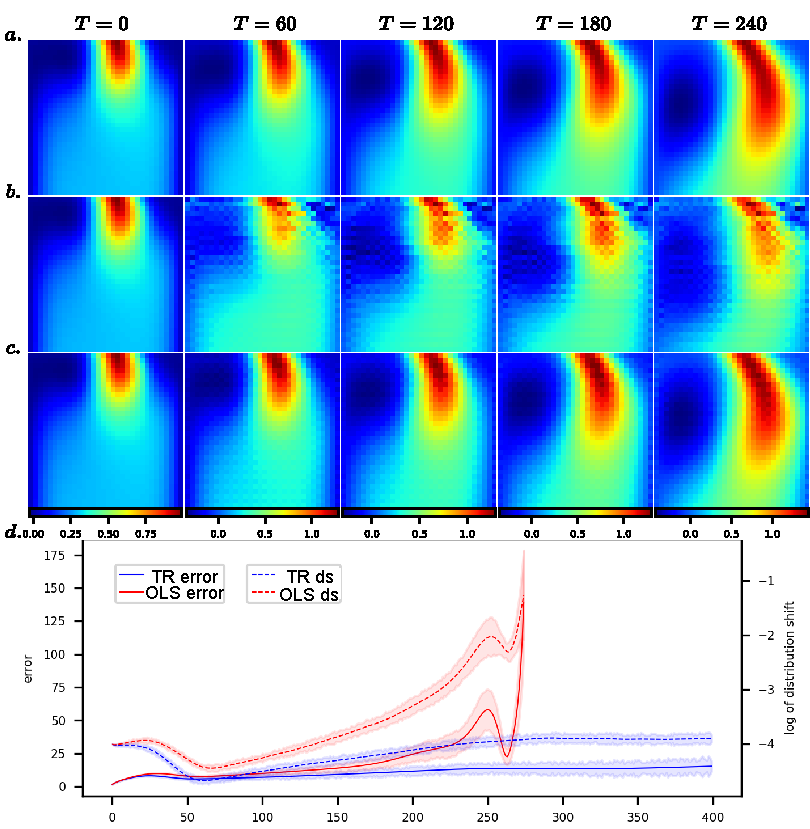
\includegraphics[width=.5\linewidth]{fig/NS-TR.pdf}}
	\end{figure}
\end{frame}

\begin{frame}{One step further: SGS modeling}
	\begin{equation*}
		\begin{aligned}
		\frac{\p u_i}{\p t} + \frac{\p}{\p x_j}(u_iu_j) & \ = 
		-\frac{\p p}{\p x_i} + \nu\Delta u_i,   \\
		\frac{\p u_i}{\p x_i} & \ = 0.
		\end{aligned}
	\end{equation*}
	Applying a filter $G$ to the equation, i.e. 
	$\overline{u} = G * u$
	\begin{equation*}
		\begin{aligned}
		\frac{\p \overline{u}_i}{\p t} + \frac{\p}{\p x_j}(\overline{u}_i
		\overline{u}_j) & \ = -\frac{\p \overline{p}}{\p x_i} + \nu\Delta 
		\overline{u}_i - \frac{\p \tau_{ij}}{\p x_j},   \\
		\frac{\p \overline{u}_i}{\p x_i} & \ = 0,		\\
		\tau_{ij} & \ = \overline{u_iu_j} - \overline{u}_i\overline{u}_j.
		\end{aligned}
	\end{equation*}
	
	{\color{red}
	\begin{equation*}
		\min_{\theta} \mbE \norml \tau - \phi_{\theta}(\overline{\mfu}) \normr^2 \Longrightarrow
		\text{Blow up simulation or wrong statistics.}
	\end{equation*}}
\end{frame}

\begin{frame}{Understanding the SGS modeling}
	Kuramoto–Sivashinsky equation:
	\begin{equation*}
		\begin{aligned}
			u_t = -(c + u)u_x - uu_x - u_{xx} - \nu u_{xxxx}, \quad u(0, t) = u(L, t) = 
			u_x(0, t) = u_x(L, t) = 0, \forall t.
		\end{aligned}
	\end{equation*}
	\begin{figure}[ht]
     \centering 
     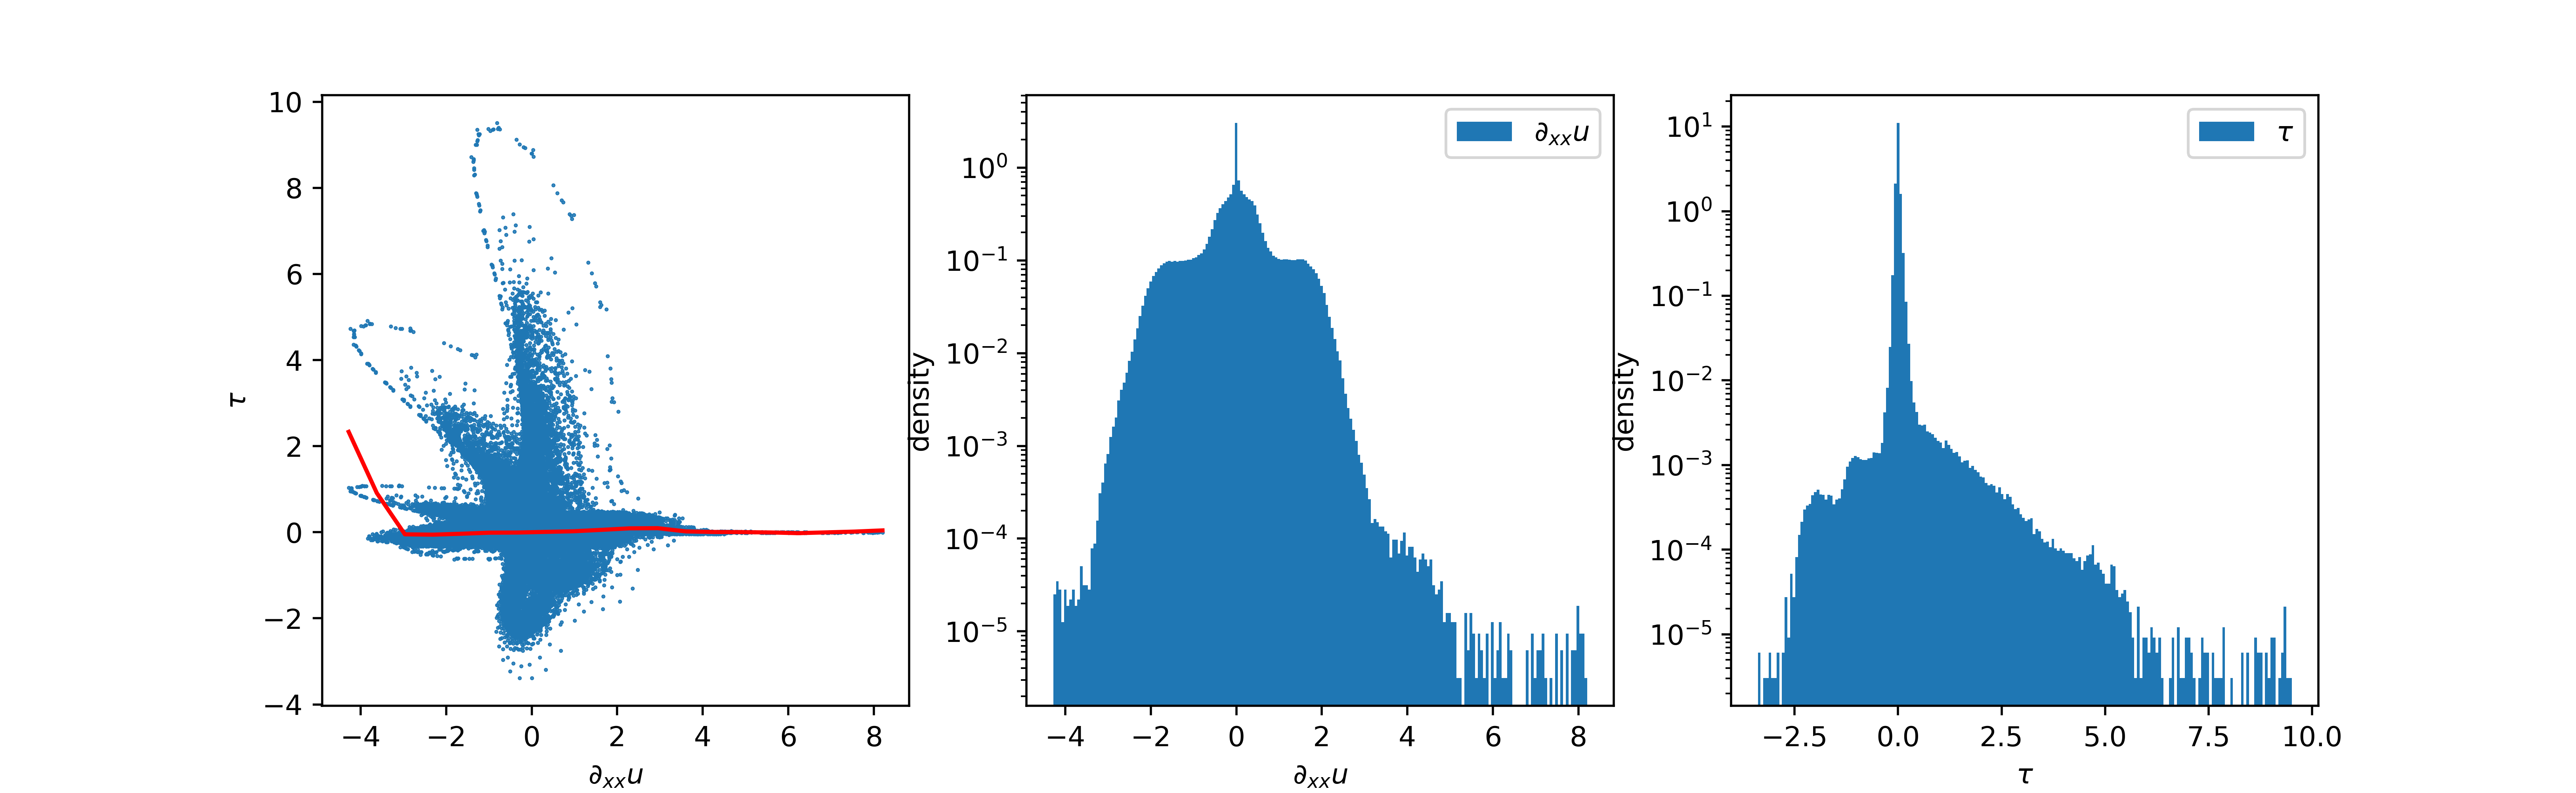
\includegraphics[width=\textwidth]
     {fig/ks_hist.png} 
\end{figure}
\hspace{2cm}\textbf{Multivaluedness}\hspace{3cm}\textbf{Data imbalance}
\end{frame}

% 1 hour talk
\begin{frame}{Understanding the SGS modeling}
	\begin{itemize}
		\item 1. {\color{red}
		Boundary layer (BL) and multiscale structure causes the data imbalance.} For
		wall-bounded NS equation:
		\begin{itemize}
			\item BL of thickness $\delta \propto \sqrt{\nu}$ $\Longrightarrow$
			$O(\nu^{-1/2})$ gradients for $O(\sqrt{\nu})$ portion of data.
			\item Bulk fluid has $O(1)$ gradients.
		\end{itemize}
		\item 2. Dimension reduction caused the multivaluedness: Mori-Zwanzig formalism.
	\end{itemize}

	Sanity check on homogeneous isotropic turbulence (HIT) data:
	\begin{figure}[ht]
     \centering
			\begin{subfigure}[b]{0.55\textwidth}
				\centering 
				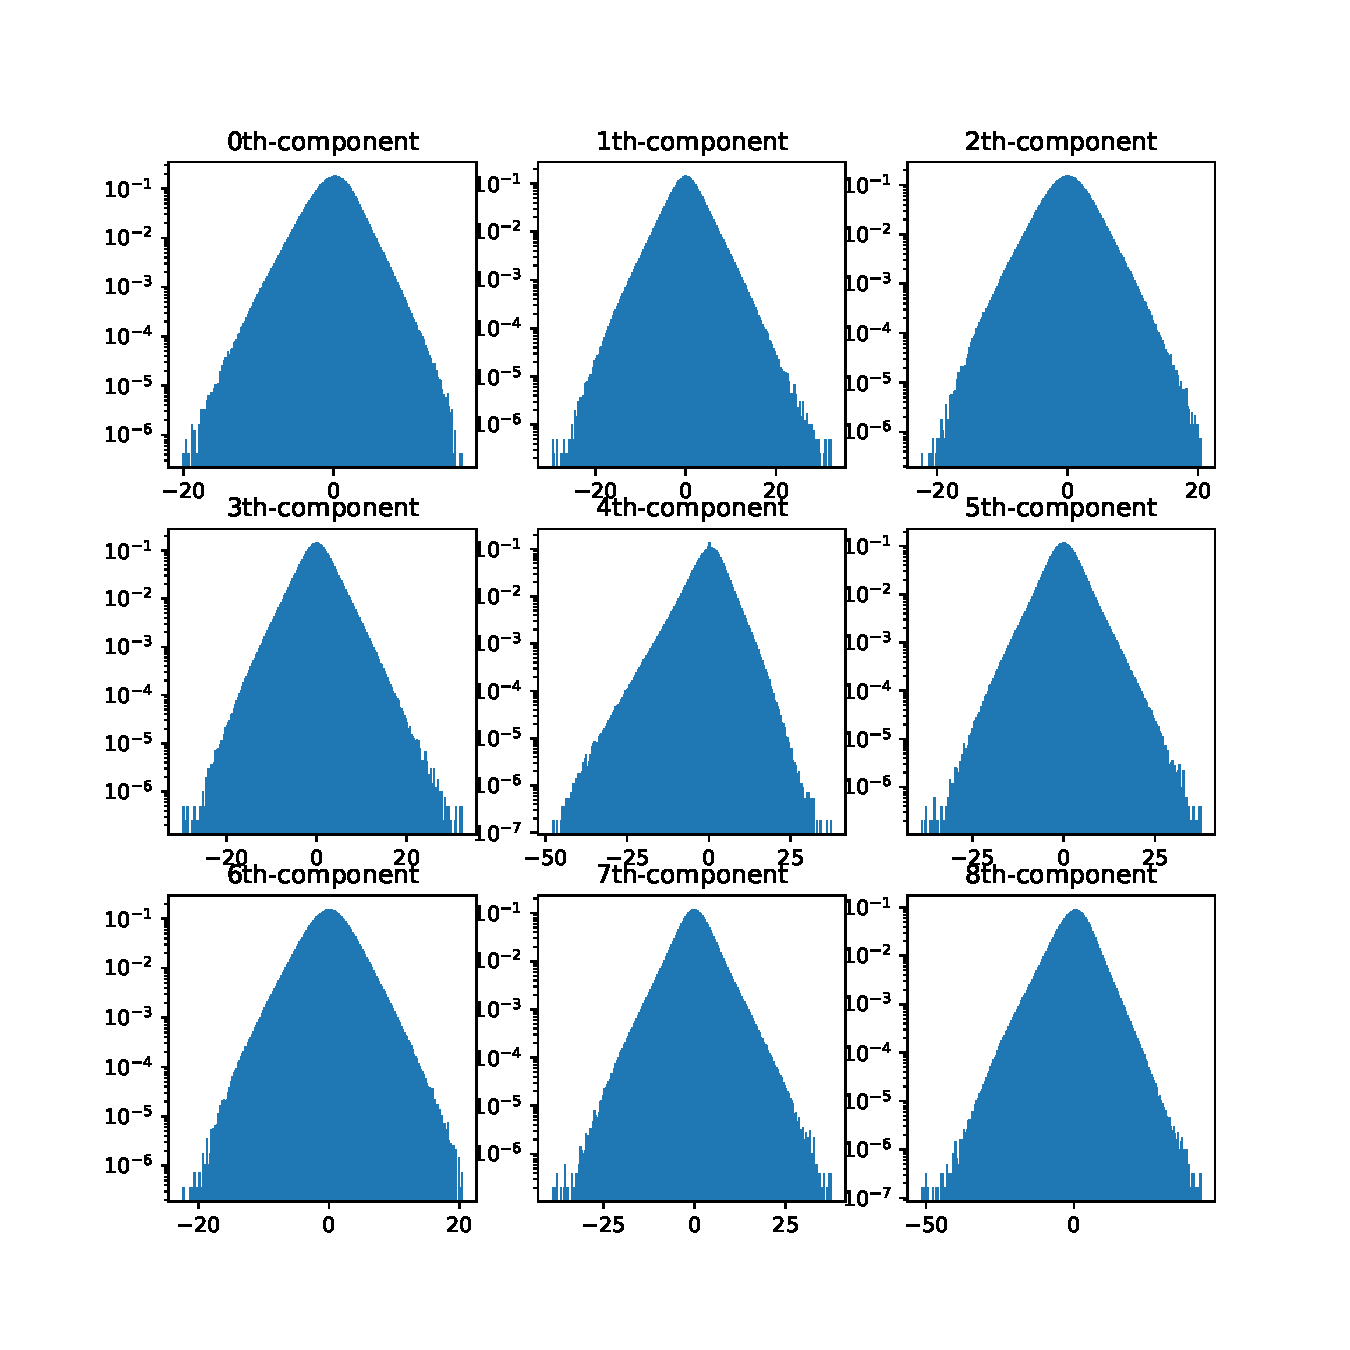
\includegraphics[width=\textwidth]
				{fig/HIT_hist_S.pdf} 
			\end{subfigure}
			\end{figure}
\end{frame}

\begin{frame}{Solution: Probabilistic ansatz}
	Regression to generative modeling:
	\begin{equation*}
    \tau = \phi_{\theta}(\mfu) \quad \rightarrow \quad \tau \sim p_{\theta}(\cdot|\mfu).
	\end{equation*}

	Change of the loss functions:
	\begin{equation*}
   \min_{\theta} \sum_{n} \norml \phi_{\theta}(\wtd{\mfu}^{(n)}) - \tau^{(n)} \normr^2,\quad
	 \max_{\theta}\sum_{i=n}^{N}\log p_{\theta}(\tau^{(n)}|\mfu^{(n)}).
	\end{equation*}
	\footnotetext[2]{Zhao, Jiaxi, Sohei Arisaka, and Qianxiao Li. 
	"Generative subgrid-scale modeling." ICLR 2025 Workshop on Machine
	Learning Multiscale Processes.}
\end{frame}


\begin{frame}{Integrating in the simulation}
	How can we deploy this model in the simulation?
	\begin{equation*}
		\begin{aligned}
			\text{Gaussian: } \mfu_i & \Longrightarrow \mu_{\theta}(\mfu_i), \sigma_{\theta}(\mfu_i),
			z \sim N(0, 1), \\
			\tau_{ij} & = \mu_{\theta}(\mfu_i) + \sigma_{\theta}(\mfu_i)z,	\\
			\text{Gaussian mixture: } \mfu_i & \Longrightarrow \mu_{\theta}^j(\mfu_i), \sigma_{\theta}^j(\mfu_i),
			z \sim N(0, 1), j \sim [M], \\
			\tau_{i} & = \mu_{\theta}^j(\mfu_i) + \sigma_{\theta}^j(\mfu_i)z,	\\
		\end{aligned}
	\end{equation*}
	There is temporal and spatial consistency issue. Should we use the same
	latent variable $z$ for all the grid points at all the time step or we
	should use different $z_i$ for different $\mfu_i$?
\end{frame}


\begin{frame}{Comparison with NN ansatz and Smagorinsky model ansatz}
	\begin{figure}[ht]
		\centering
		\begin{subfigure}[b]{0.32\textwidth}
			\centering 
			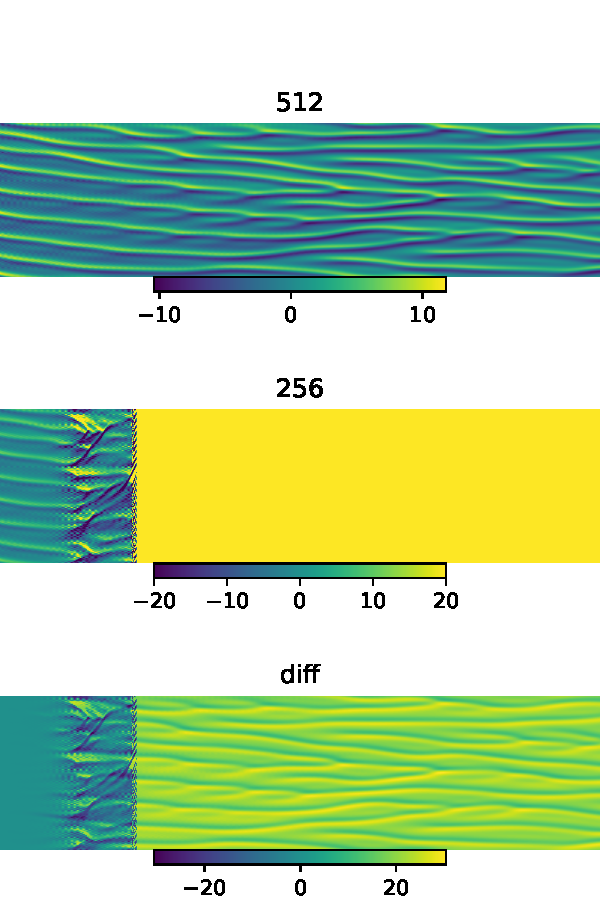
\includegraphics[width=\textwidth]
			{fig/ks_nu0.1_N1512N2256_correct_cmp_lr1e-4.pdf} 
			\caption{Regression ansatz: neural network} 
		\end{subfigure}
		\begin{subfigure}[b]{0.32\textwidth}
			\centering 
			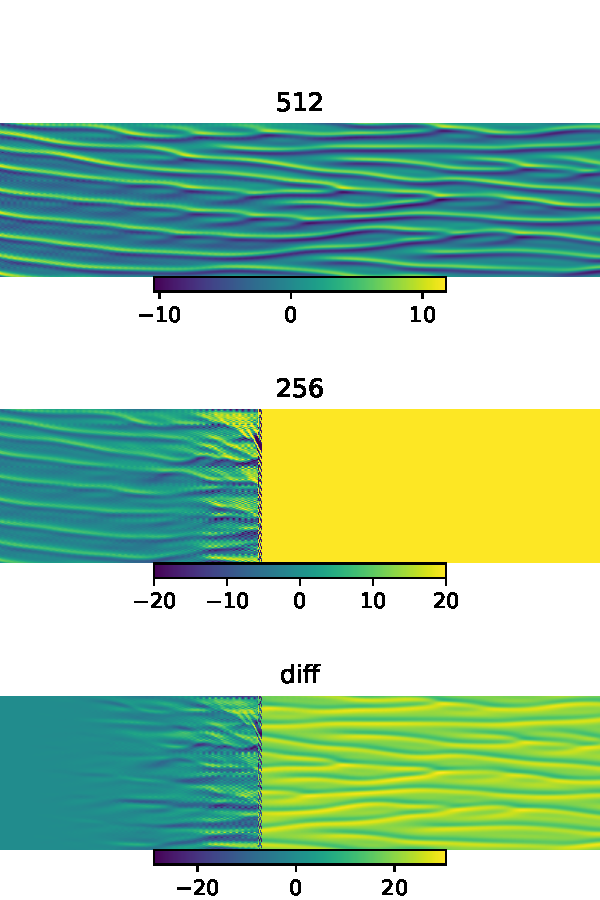
\includegraphics[width=\textwidth]{fig/ks_nu0.1_N1512N2256_correct_cmp_lr2e-4.pdf} 
			\caption{Regression ansatz: Smagorinsky} 
		\end{subfigure}
		\begin{subfigure}[b]{0.32\textwidth}
			\centering 
			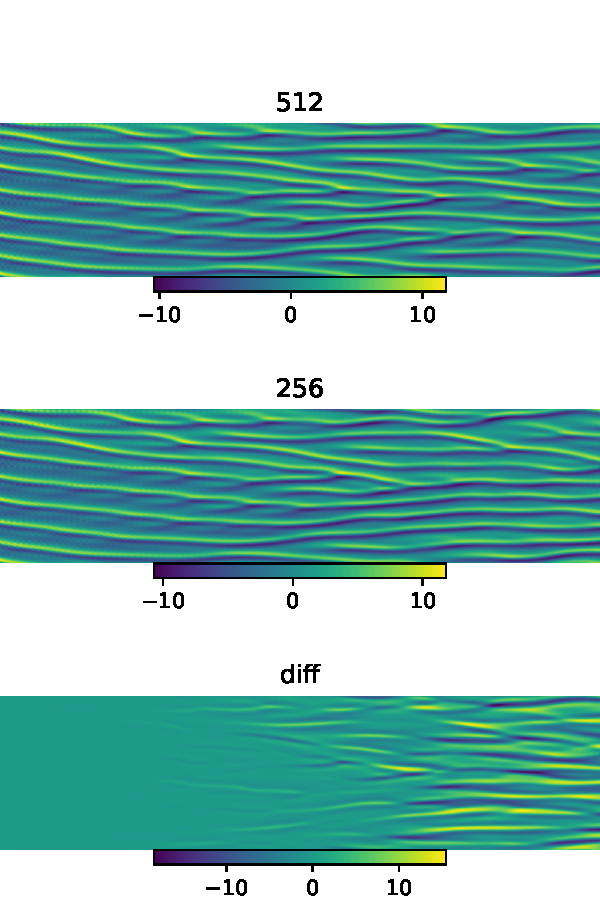
\includegraphics[width=\textwidth]{fig/ks_nu0.1_N1512N2256_correct_cmp_lr5e-4.pdf} 
			\caption{Probabilistic ansatz: Gaussian}  
		\end{subfigure}
	\end{figure}
\end{frame}


\begin{frame}{Comparison with the regression-based method}
	\begin{equation*}
		\begin{aligned}
			\la\overline{u}\ra &= \frac{1}{LT}\int_{[0, L]}\int_{t}^{t+T} u(x, t)dt dx,
			\\
			\la\overline{u^2}\ra &= \frac{1}{LT}\int_{[0, L]}\int_{t}^{t+T}
			u^2(x, t)dt dx, \\
		\end{aligned}
	\end{equation*}
	\begin{figure}[ht]
		\centering
		\begin{subfigure}[b]{0.38\textwidth}
				\centering
				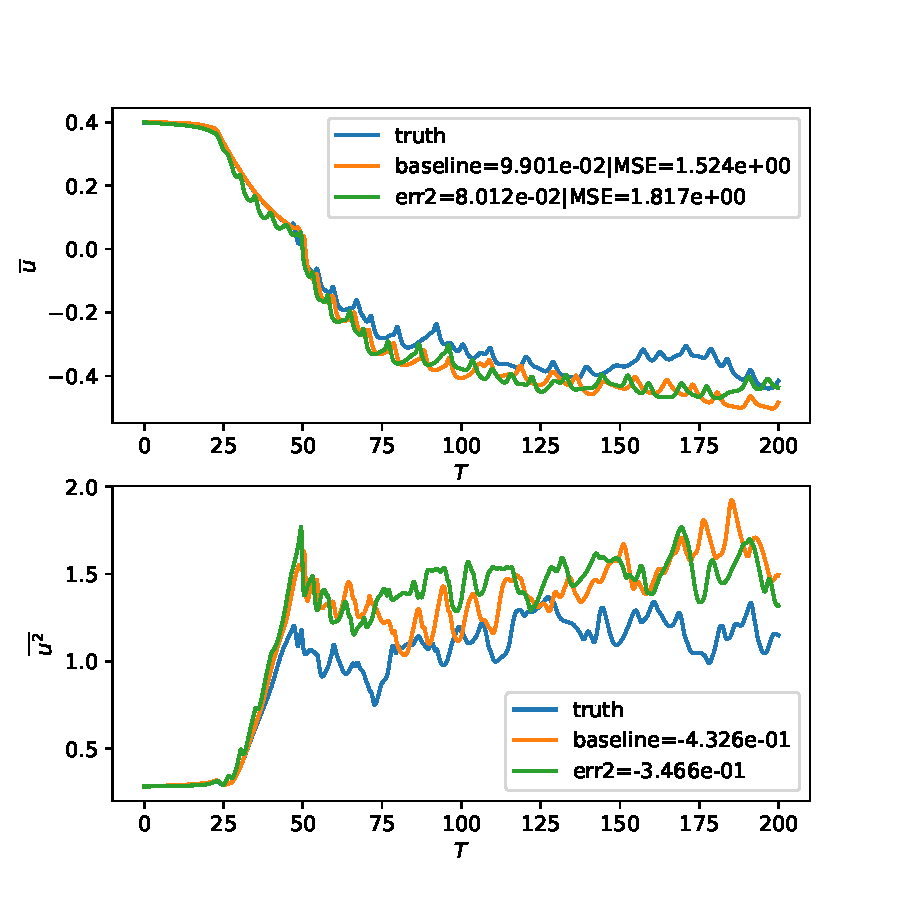
\includegraphics[width=\textwidth]
				{fig/ks_nu1_N1023n10_regression_cmp_stats.pdf}
		\end{subfigure}
		\begin{subfigure}[b]{0.38\textwidth}
				\centering
				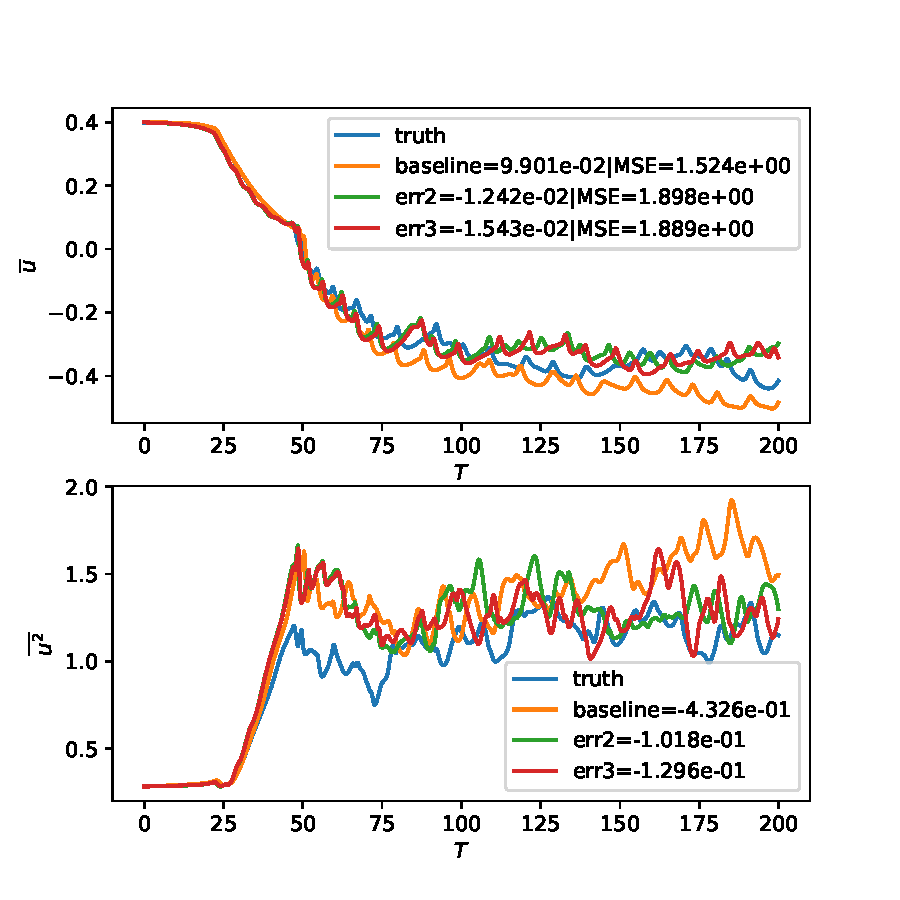
\includegraphics[width=\textwidth]
				{fig/ks_nu1_N1023n10_gaussian_cmp_stats.pdf}
		\end{subfigure}
		\label{fig:cmp_stats1}
	\end{figure}
\end{frame}


\begin{frame}{Code development}

	\url{https://github.com/jiaxi98/ml4dynamics}

	\textit{A codebase for testing various algorithms for data-driven hybrid simulations,}
	\begin{itemize}
		\item 1. Regularization-based method.
		\item 2. Generative modeling.
		\item 3. Active-learning method.
	\end{itemize}

	
	\url{https://github.com/jiaxi98/pyfoam}

	\textit{Data-driven turbulence modeling platform based on OpenFOAM.}
\end{frame}


\begin{frame}{Backup slides}
	\begin{figure}[ht] 
		\centering 
		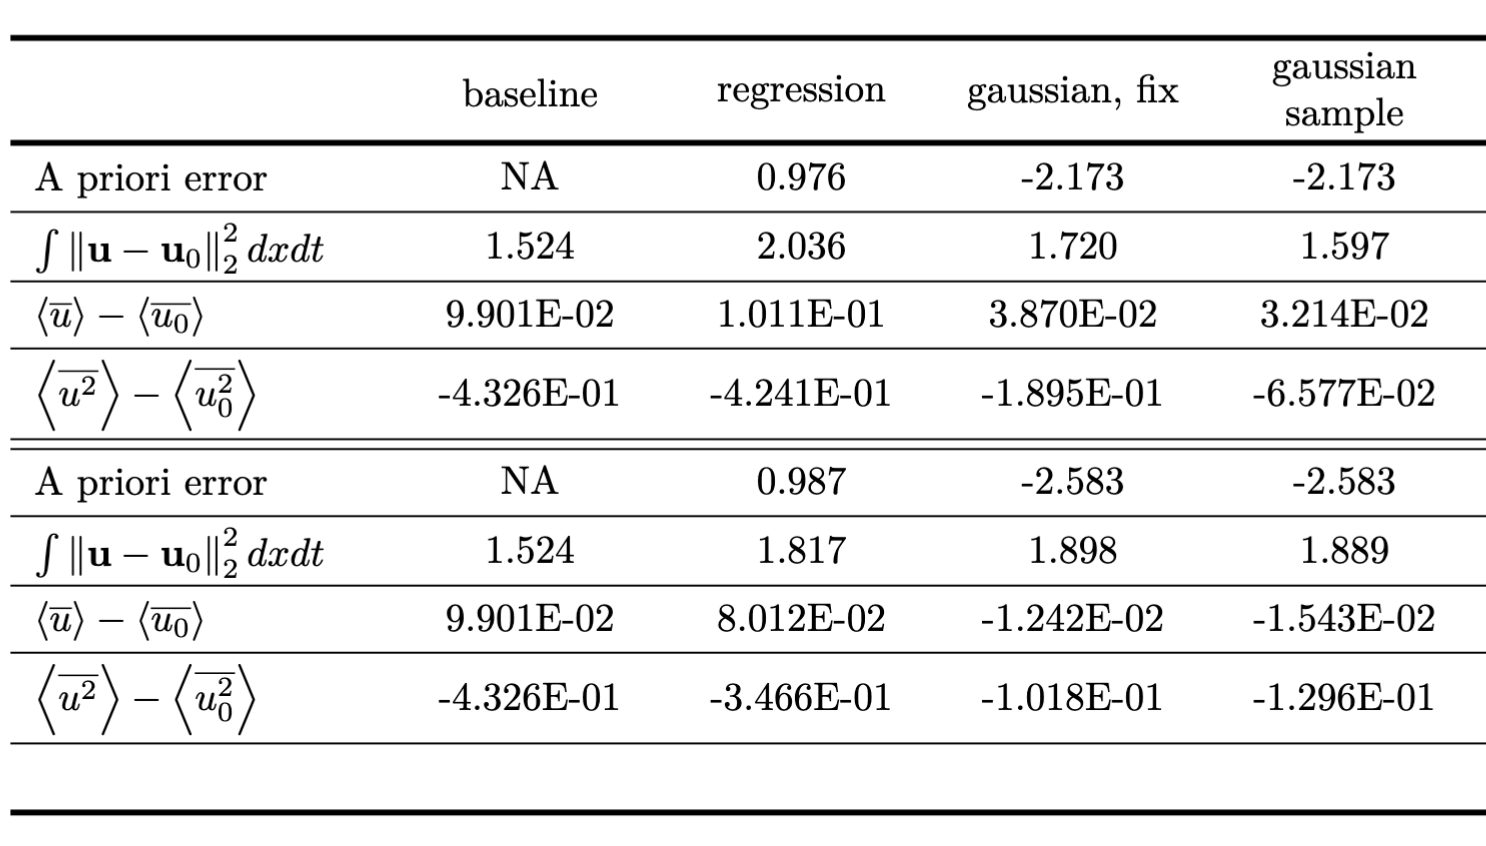
\includegraphics[width=\textwidth]{fig/table.jpg} 
	\end{figure}
\end{frame}


\begin{frame}{Backup slides}
	\begin{figure}[ht] 
		\centering 
		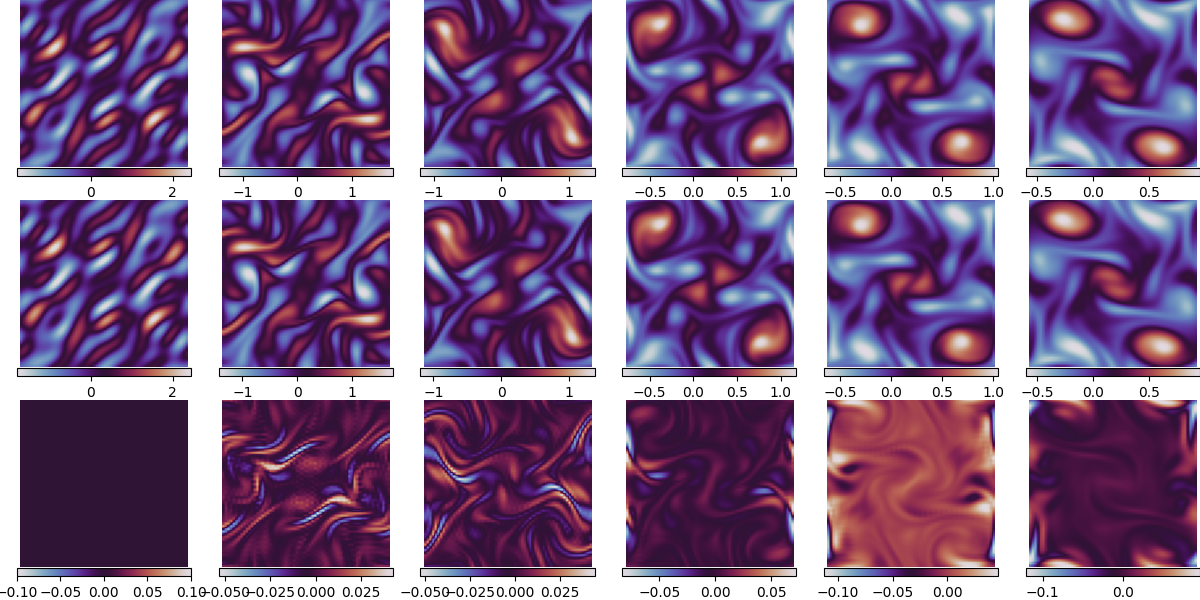
\includegraphics[width=\textwidth]{fig/sim_ns_hit_coarse_correction_ols_unet.png} 
	\end{figure}
\end{frame}


\begin{frame}{Backup slides}
	\begin{figure}[ht] 
		\centering 
		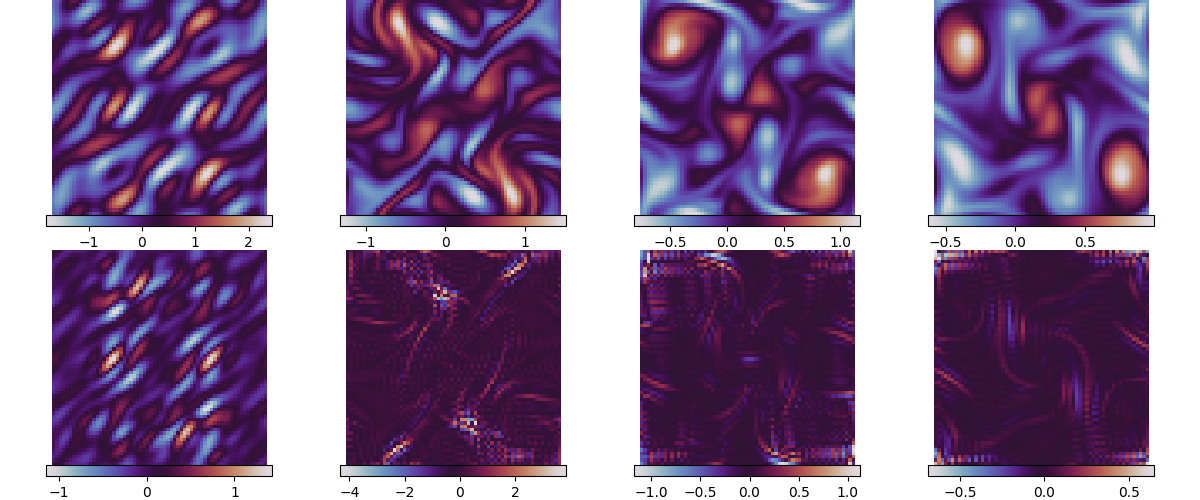
\includegraphics[width=\textwidth]{fig/dataset_filter.png} 
	\end{figure}
\end{frame}

\end{document}